\documentclass[a4paper,11pt]{article}[24.3.2010]
\usepackage[left=2cm,top=3cm,text={17cm, 24cm}]{geometry}
\usepackage{amsthm}
\usepackage{times}
\usepackage{amsfonts}
\usepackage{amsmath}
\usepackage{graphics}
\usepackage{picture}
\usepackage{eurosym}
\usepackage{lastpage}
\usepackage[czech]{babel}
\usepackage[utf8]{inputenc}
\usepackage{fancyhdr}
\usepackage{skull}
\usepackage{color}
\pagestyle{fancy}
\newcommand\myuv[1]{\quotedblbase #1\textquotedblleft}
\author{Jan Vybíral\\xvybir05@stud.fit.vutbr.cz}
\title{Typografie a publikování -- 1. projekt}
\date{}
\cfoot{\thepage\//\pageref{LastPage}}
\rhead{\textbf{Jan Vybíral, XVYBIR05}}

 
\begin{document}





\begin{enumerate}
\item Rozhodněte, zda je třída \emph{rekurzivních} jazyků uzavřena vůči inverznímu morfismu. Popište ideu důkazu, podobně jako je tomu u věty 8.4 na přednáškách (můžete použít vícepáskový Turingův stroj).\\

Ano, třída rekurzivních jazyků je uzavřena vůči inverznímu morfismu.\\

Idea důkazu:

\begin{itemize}
\item Aby byla třída rekurzivních jazyků uzavřená vůči inverznímu morfismu, musí platit, že pro každý rekurzivní jazyk $L_{1}\subseteq\Sigma_{1}^*$ a pro každý morfismus $h : \Sigma_{2}^* \rightarrow \Sigma_{1}^*$ je $L_{2} = h^{-1}(L_{1}) \subseteq \Sigma_{2}^*$ také rekurzivní jazyk.\\
\item Jazyk $L\subseteq\Sigma^*$ je rekurzivní, jestliže $L=L(M)$ pro nějaký úplný Turingův stroj $M$.\\
\item Z předchozích dvou bodů plyne, že třída rekurzivních jazyků je uzavřena vůči inverznímu morfismu, pokud je možné pro každý rekurzivní jazyk $L_{1}\subseteq\Sigma_{1}^*$ a pro každý morfismus $h : \Sigma_{2}^* \rightarrow \Sigma_{1}^*$ sestavit úplný Turingův stroj $M_{2}$ takový, že $L(M_{2})=L_{2} = h^{-1}(L_{1}) \subseteq \Sigma_{2}^*$.\\
\item Z definic morfismu jazyka a inverzního morfismu jazyka ve studijní opoře plyne, že musí také platit:\\
$w \in L_{2} \Leftrightarrow h(w) \in L_{1}$.\\

\item $M_{2}$ lze sestrojit takto:\\
\begin{itemize}
\item Pro morfismus $h : \Sigma_{2}^* \rightarrow \Sigma_{1}^*$ můžeme definovat funkci $h_{0} : \Sigma_{2} \rightarrow \Sigma_{1}^*$ takovou, že $h_{0}(a) = h(a)$ a $h(w) = h_{0}(a_{1})h_{0}(a_{2})...h_{0}(a_{n})$.\\
\item Protože množina $\Sigma_{2}$ je konečná, tak $h_{0}$ může být zakódována v řízeni $M_{2}$.\\
\item Z výše uvedené ekvivalence plyne, že dvoupáskový $M_{2}$ může pracovat tak, že pro vstupní řetězec $w \in \Sigma_{2}^*$ na první pásce uloží na druhou pásku řetězec $h(w) \in \Sigma_{1}^*$ (postupně prochází vstup na první pásce a pro každý znak $a$ uloží na korespondující pozici na druhé pásce $h_{0}(a)$). Poté na druhé pásce simuluje běh stroje $M_{1}$. Pokud ten přijme, přijme i $M_{2}$.\\
\end{itemize}
\item Je zřejmé, že pokud je $M_{1}$ úplný, $M_{2}$ musí také být úplný. Třída rekurzivních jazyků tudíž je uzavřena vůči inverznímu morfismu.
\end{itemize}

\newpage

\item Uvažujte jazyk $L_{LOA}$ kódů lineárně omezených Turingových strojů (t.j., jazyk kódů Turingových strojů takových, že v žádném jejich výpočtu neopustí vstupní hlava oblast pásky, na které bylo zapsáno vstupní slovo). Dokažte redukcí, že $L_{LOA}$ není RE. Může vám pomoci následující nápověda.
\renewcommand{\theenumi}{\alph{enumi}}
\begin{enumerate}
\item Co víte o problému prázdnosti jazyka Turingova stroje?
\item Pro libovolný TS $T$ můžeme sestrojit TS $T'$, který na vstupu očekává vstupní slovo $w$ stroje $T$ následované vyznačeným úsekem použitelné pásky. Bude simulovat výpočet $T$ na $w$ a vhodně zareaguje, když simulovaný výpočet $T$ skončí a také když simulace $T$ vede k opuštění vyznačeného úseku pásky.
\end{enumerate}
\renewcommand{\theenumi}{\arabic{enumi}}
Popis stroje $T'$ je v nápovědě záměrně neformální a nejednoznačný. V důkazu svou verzi stroje $T'$ definujte přesněji, nemusíte detailně popisovat redukci, ale musí být jasné, co $T'$ dělá a že jde opravdu o redukci.

\begin{itemize}
\item Použijeme redukci z problému prázdnosti jazyka Turingova stroje, který je charakterizován jazykem $L_{EMP} = \{\langle M\rangle\ \mid M$ je TS takový, že $L(M) = \emptyset\}$. Tento problém není ani částečně rozhodnutelný (viz. kapitola 6.4.2 ve studijní opoře) a tudíž jemu odpovídající jazyk $L_{EMP}$ není ani rekurzivně vyčíslitelný.
\item $L_{LOA} = \{\langle M\rangle \mid M$ je lineárně omezený TS$\}$.
\item Sestrojíme redukci $\delta : \{0,1\}^* \rightarrow \{0,1\}^*$ z jazyka $L_{EMP}$  na jazyk $L_{LOA}$. Musí platit:\\
$\forall w \in \{0,1\}^* : w \in L_{EMP} \Leftrightarrow \delta(w) \in L_{LOA}$
\item Úplný TS $M_{\delta}$ implementující redukci $\delta$ přiřadí každému řetězci $x \in \{0,1\}^*$ řetězec $\langle M_{x}\rangle$, kde $M_{x}$ je TS, který na vstupu $w \in \{0,1\}^*$ pracuje takto:
\begin{itemize}
\item Pokud $x$ není platný kód TS, $M_{x}$ bude posouvat svojí hlavu směrem doprava až na první výskyt symbolu $\Delta$ a poté přijme.
\item Jinak $M_{x}$ projde svůj vstup $w$ a zkontroluje, zda má strukturu $v\omega^k\#$, kde $v$ je platný kód vstupu TS s kódem $x$, $\omega$ a $\#$ jsou speciální zásobníkové symboly nepatřící do zásobníkové abecedy TS s kódem $x$ a $k\geq 0$ je celé číslo. Pokud ne, $M_{x}$ odmítne.\\
(tento krok by neměl způsobit, aby se čtecí hlava $M_{x}$ dostala mimo oblast na pásce, kde je zapsaný vstup, jinak důkaz nebude fungovat, ale pokud na vstupu např. je pouze $v$ bez speciálních symbolů, tak $M_{x}$ při kontrole nutně vyjede ze vstupu, tudíž ani nemůže být lineárně omezený, ale nevím, co s tím)
\item Jinak $M_{x}$ s využitím univerzálního TS $M_{u}$, který je jeho komponentou, simuluje běh TS s kódem $x$ na vstupu $w$, přičemž k speciálním symbolům $\omega$ se chová, jako by to byly symboly $\Delta$, a pokud se jeho hlava dostane nad symbol $\#$, $M_{u}$ zastaví a odmítne.
\item Pokud $M_{u}$ odmítne, odmítne i $M_{x}$.
\item Pokud $M_{u}$ přijme, $M_{x}$ bude posouvat svojí hlavu směrem doprava až na první výskyt symbolu $\Delta$ a poté přijme.
\end{itemize}
\item $\delta$ lze evidentně implementovat s pomocí úplného TS $M_{\delta}$. Stačí, aby vypsal kód TS zahrnujícího test členství $x$ v regulárním jazyce dobře zformovaných kódů TS, test členství $w$ v regulárním jazyce platných kódů vstupu TS s kódem $x$ konkatenovaných s  $\omega^*\#$ , univerzální TS $M_{u}$ a jeho aplikaci na $w$.
\item Pro TS $M_{x}$ platí:
\begin{itemize}
\item $\langle M_{x}\rangle \in L_{LOA} \Leftrightarrow$ $x$ je platný kód TS a zároveň pro všechna možná $w$ platí, že se hlava TS $M_{u}$ simulujícího běh TS s kódem $x$ na vstupu $w$ dostane nad symbol $\#$ nebo $M_{u}$ odmítne nebo cyklí, aniž by se jeho hlava dostala nad symbol $\#$. Tato varianta je zřejmě ekvivalentní tomu, že TS s kódem $x$ při jakémkoli vstupu buď odmítne nebo cyklí.
\item $\langle M_{x}\rangle \notin L_{LOA} \Leftrightarrow$ $x$ není platný kód TS nebo existuje nějaké $w$ takové, že TS $M_{u}$ simulující běh TS s kódem $x$ na vstupu $w$ přijme. Tato varianta je zřejmě ekvivalentní tomu, že TS s kódem $x$ přijímá alespoň jedno slovo.
\end{itemize}
\item Ukážeme, že $\delta$ zachovává členství v jazyce dle definice redukce:\\
$\forall x \in \{0,1\}^* : x \in L_{EMP} \Leftrightarrow$ TS s kódem $x$ nepřijímá žádné slovo $\Leftrightarrow \langle M_{x}\rangle \in L_{LOA}$
\item Tedy $L_{LOA}$ není ani rekurzivně vyčíslitelný.
\end{itemize}

\newpage

\item Uvažujte následujíci dva důkazy diagonalizací. Oba jsou chybné (ani jedno z dokazovaných tvrzení neplatí). Vysvětlete, který krok je chybný a zdůvodněte proč. Může vám pomoci důkladně si prostudovat kapitolu o diagonalizaci ve studijní opoře. Nehledejte komplikovaná řešení, ke zdůvodnění by vám měla stačit jedna až dvě věty.
\renewcommand{\theenumi}{\alph{enumi}}
\begin{enumerate}
\item Důkaz, že množina $A \subseteq 2^{\{0\}^*}$ všech \emph{konečných} jazyků nad abecedou $\{0\}$ má jinou mohutnost než množina $B \subseteq 2^{\{0,1\}^*}$ všech \emph{konečných} jazyků nad abecedou $\{0,1\}$.
\begin{enumerate}
\item Předpokládejme, že $A$ i $B$ mají stejnou mohutnost. Pak existuje bijekce $f : A \rightarrow B$.
%\textcolor{green}{OK: http://cs.wikipedia.org/wiki/Mohutnost}
\item Prvky množiny $A$ je možné očíslovat přirozenými čísly a seřadit do posloupnosti $L_{1},L_{2},L_{3},...$.
%\textcolor{green}{OK: $A$ je spočetná, protože $\overline{L}$ musí být nekonečné a $A$ je množina konečných jazyků.}
\item Slova z množiny $\{0,1\}^*$ je taktéž možno uspořádat do nějaké posloupnosti $w_{1},w_{2},w_{3},...$ (například lexikograficky).
%\textcolor{green}{OK: viz. opora.}
\item $f$ potom můžeme zobrazit nekonečnou maticí $m$, kde $m_{ij}$ je $1$, pokud $w_{j} \in f(L_{i})$, a $0$ jinak:
\begin{table}[ht]
\begin{center}
\begin{tabular}{ c  c  c  c  c } 
& $w_{1}$ & $w_{2}$ & $w_{3}$ & $...$ \\ 
$f(L_{1})$ & $1$ & $0$ & $1$ & $...$ \\ 
$f(L_{2})$ & $0$ & $0$ & $1$ & $...$ \\ 
$f(L_{3})$ & $1$ & $1$ & $1$ & $...$ \\ 
$...$ & $...$ & $...$ & $...$ & $...$ \\
\end{tabular}
\end{center}
\end{table}
%\textcolor{green}{OK: viz. opora.}
\item Uvažujme jazyk $L \subseteq \{0,1\}^*$, který vznikne komplementací diagonály, tedy takový, že pro každé $i>0,w_{i} \in L$, právě když $w_{i} \notin f(L_{i})$ (tedy právě když $m_{ii}=0$).
%\textcolor{green}{OK: viz. opora.}
\item Jazyk $L$ se zřejmě liší od každého jazyka $f(L_{i}),i>0$  (alespoň slovem $w_{i}$).
%\textcolor{green}{OK: viz. opora.}
\item Zároveň je jazyk $L$ v $B$.
\item To ale znamená, že $f$ není surjektivní, a tedy nemůže být bijekcí. Spor.\\
\end{enumerate}
Krok vii. je chybný! Jelikož je matice nekonečná, i $L$ je nekonečný, tudíž nemůže patřit do množiny konečných jazyků $B$!\\
\item Stejné tvrzení a stejný důkaz jako v bodě 3a, pouze s tím rozdílem, že nyní $A = 2^{\{0\}^*}$ a $B = 2^{\{0,1\}^*}$, t.j., $A$ i $B$ teď obsahují všechny jazyky nad danými abecedami, včetně \emph{nekonečných}.\\

Krok ii. je chybný! $A$ je nespočetná, viz. Lemma 6.1.1. ve studijní opoře, tudíž její prvky nelze očíslovat přirozenými čísly a seřadit do posloupnosti $L_{1},L_{2},L_{3},...$.

\end{enumerate} 
\renewcommand{\theenumi}{\arabic{enumi}}

\newpage

\item Na Obrázku $1$ je zobrazen dvoupáskový NTS \emph{Happy End}, který přijímá jednoduchý regulární jazyk nad abecedou $\Sigma=\{N,T,I,\heartsuit,\skull,?,!\}$. Jaký?\\\\
Demonstrujte běh \emph{Happy End} na nějakém slově z $L$(\emph{Happy End}) (stačí, když uvedete konfigurace druhé pásky na vstupu každého uzlu z obrázku $1$, kterým běh stroje prochází). 

\begin{figure}[htbp]
  \centering
  \scalebox{0.23}{
   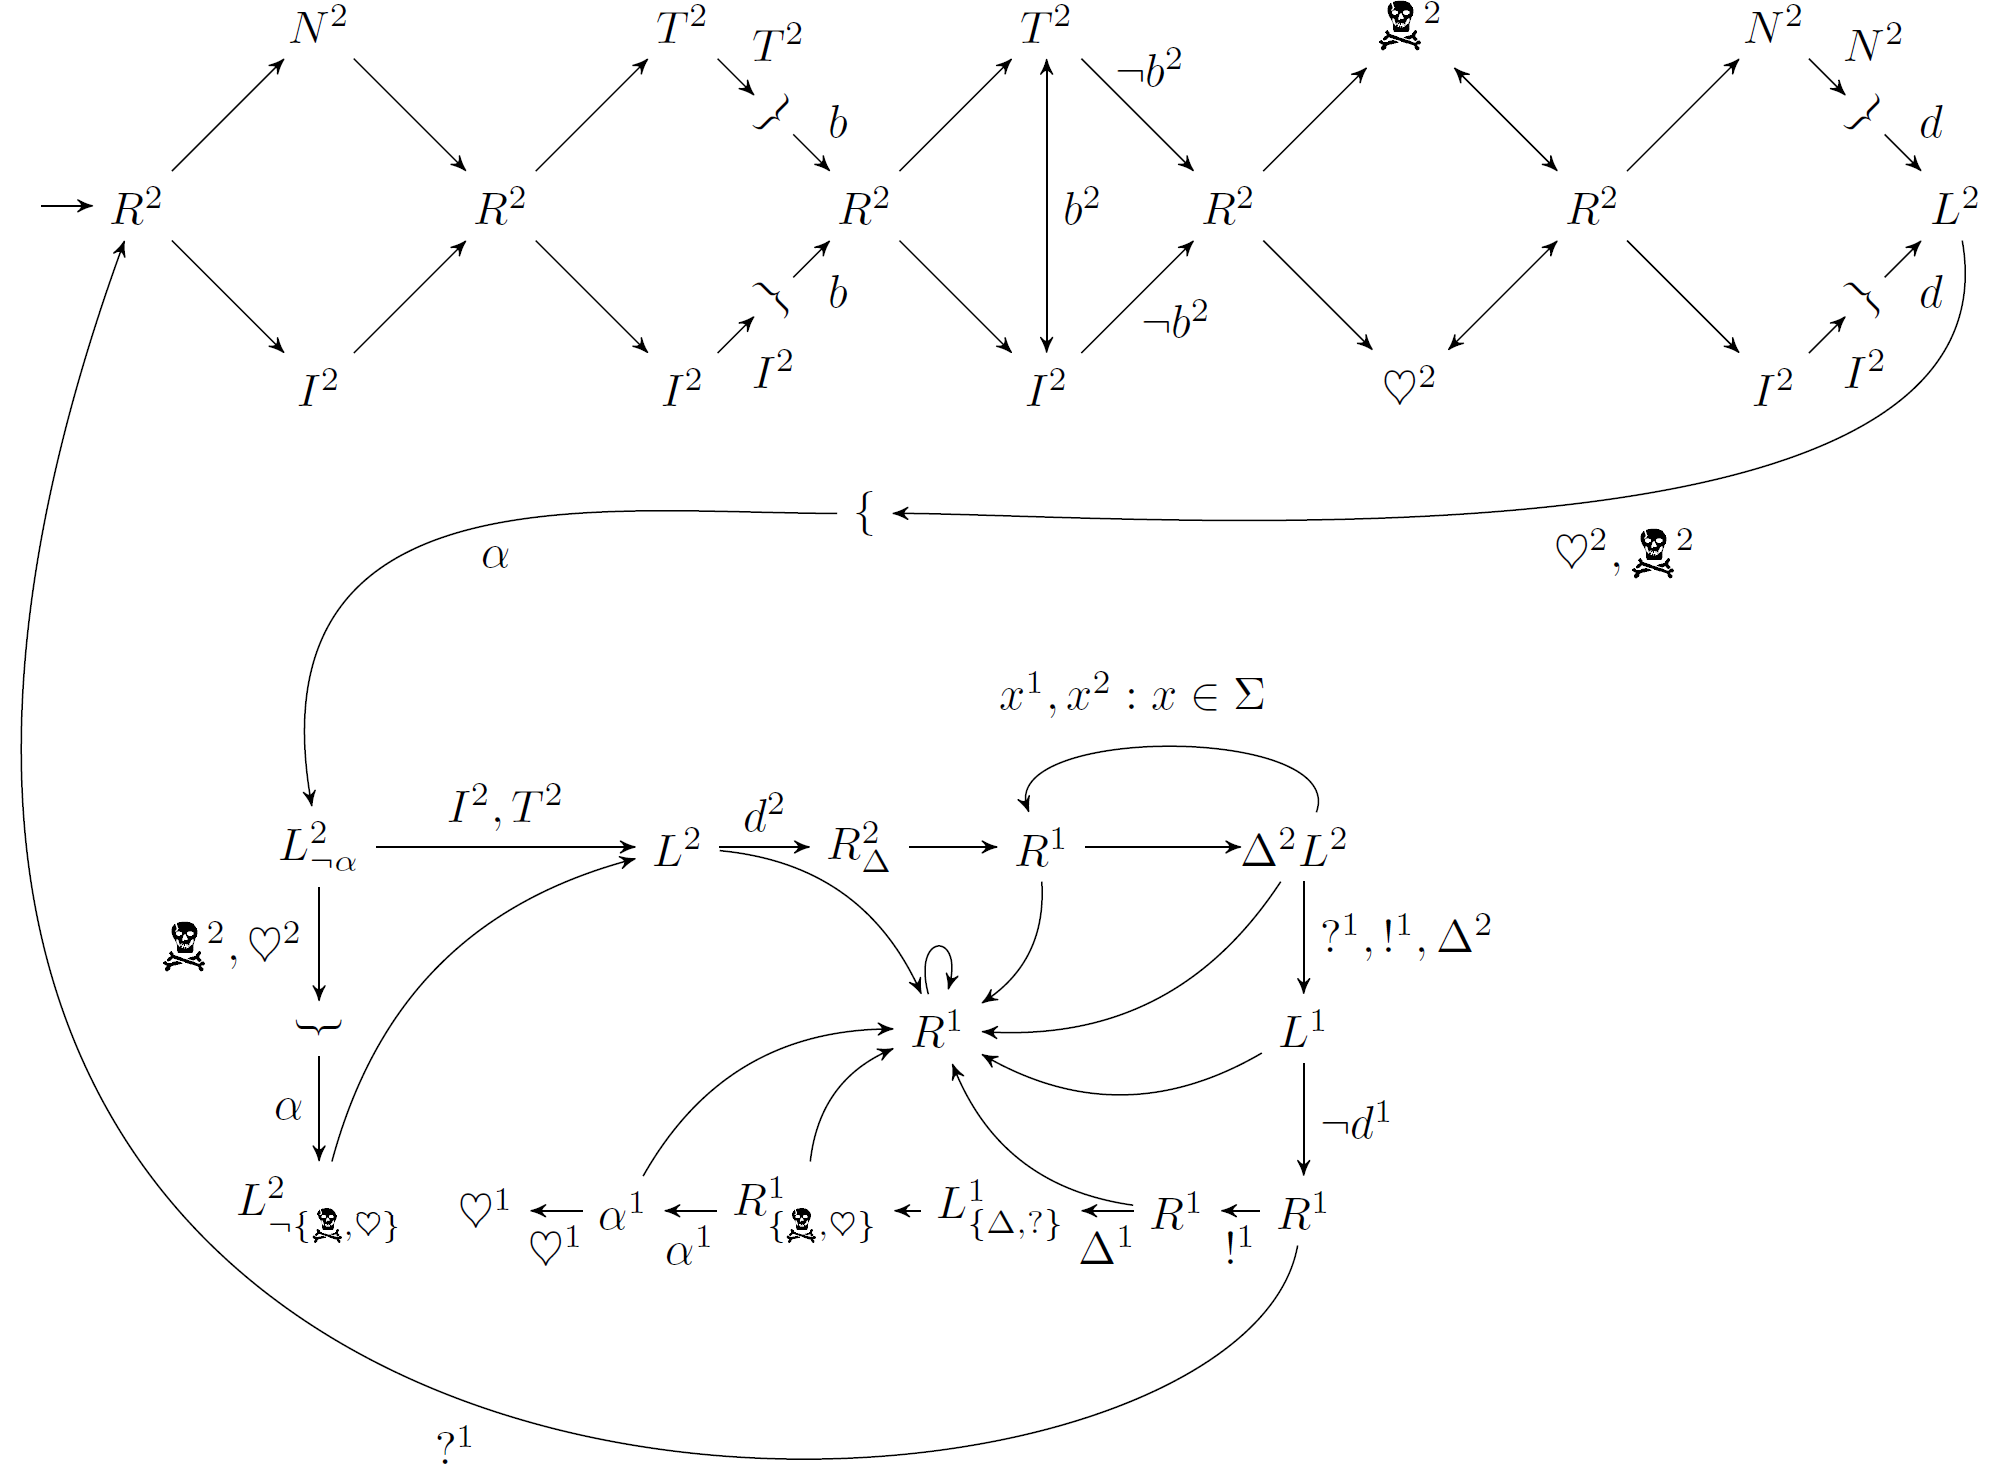
\includegraphics{img/NTS.png}
   }
  \caption{NTS \emph{Happy End}.}
\end{figure} 

NTS \emph{Happy End} přijímá regulární jazyk ekvivalentní regulárnímu výrazu: $(I(\heartsuit+\skull)^+TIN?)^*  I\heartsuit^+TIN!$\\

Posloupnost konfigurací druhé pásky NTS \emph{Happy End} na vstupu každé jeho komponenty, kterou prochází jeho běh, který přijme slovo $I\heartsuit TIN!$:

\begin{table}[ht]
        \begin{center}
        \begin{tabular}{ l  l  l  l  l  l } 
        %1.&$[\textcolor{red}{\underline{\Delta}}\Delta\ldots]$ & 15.&$[\Delta NIT\heartsuit I \textcolor{red}{\underline{\Delta}}\ldots]$ & 29.&$[\Delta N\textcolor{red}{\underline{\Delta}}\Delta\Delta\Delta\Delta\ldots]$\\
        %2.&$[\Delta\textcolor{red}{\underline{\Delta}}\Delta\ldots]$ & 16.&$[\Delta NIT\heartsuit I \textcolor{red}{\underline{\Delta}}\ldots]$ & 30.&$[\Delta \textcolor{red}{\underline{N}}\Delta\Delta\Delta\Delta\Delta\ldots]$\\
        %3.&$[\Delta\textcolor{red}{\underline{N}}\Delta\ldots]$ & 17.&$[\Delta NIT\heartsuit I \textcolor{red}{\underline{\Delta}}\ldots]$ & 31.&$[\Delta \textcolor{red}{\underline{N}}\Delta\Delta\Delta\Delta\Delta\ldots]$\\
        %4.&$[\Delta N\textcolor{red}{\underline{\Delta}}\ldots]$ & 18.&$[\Delta NIT\heartsuit\textcolor{red}{\underline{I}}\Delta\ldots]$ & 32.&$[\Delta \textcolor{red}{\underline{\Delta}}\Delta\Delta\Delta\Delta\Delta\ldots]$\\
        %5.&$[\Delta N\textcolor{red}{\underline{I}}\Delta\ldots]$ & 19.&$[\Delta NIT\heartsuit\textcolor{red}{\underline{I}}\Delta\ldots]$ & 33.&$[\textcolor{red}{\underline{\Delta}}\Delta\Delta\Delta\Delta\Delta\Delta\ldots]$\\
        %6.&$[\Delta NI\textcolor{red}{\underline{\Delta}}\ldots]$ & 20.&$[\Delta NIT\heartsuit\textcolor{red}{\underline{\Delta}}\Delta\ldots]$ & 34.&$[\textcolor{red}{\underline{\Delta}}\Delta\Delta\Delta\Delta\Delta\Delta\ldots]$\\
        %7.&$[\Delta NI\textcolor{red}{\underline{T}}\Delta\ldots]$ & 21.&$[\Delta NIT\textcolor{red}{\underline{\heartsuit}}\Delta\Delta\ldots]$ & 35.&$[\textcolor{red}{\underline{\Delta}}\Delta\Delta\Delta\Delta\Delta\Delta\ldots]$\\
        %8.&$[\Delta NIT\textcolor{red}{\underline{\Delta}}\ldots]$ & 22.&$[\Delta NIT\textcolor{red}{\underline{\heartsuit}}\Delta\Delta\ldots]$ & 36.&$[\textcolor{red}{\underline{\Delta}}\Delta\Delta\Delta\Delta\Delta\Delta\ldots]$\\
        %9.&$[\Delta NIT\textcolor{red}{\underline{\heartsuit}}\Delta\ldots]$ & 23.&$[\Delta NIT\textcolor{red}{\underline{\Delta}}\Delta\Delta\ldots]$ & 37.&$[\textcolor{red}{\underline{\Delta}}\Delta\Delta\Delta\Delta\Delta\Delta\ldots]$\\
        %10.&$[\Delta NIT\heartsuit\textcolor{red}{\underline{\Delta}}\ldots]$ &24.&$[\Delta NI\textcolor{red}{\underline{T}}\Delta\Delta\Delta\ldots]$ &38.&$[\textcolor{red}{\underline{\Delta}}\Delta\Delta\Delta\Delta\Delta\Delta\ldots]$\\
        %11.&$[\Delta NIT\heartsuit\textcolor{red}{\underline{I}}\Delta\ldots]$ & 25.&$[\Delta NI\textcolor{red}{\underline{T}}\Delta\Delta\Delta\ldots]$ &39.&$[\textcolor{red}{\underline{\Delta}}\Delta\Delta\Delta\Delta\Delta\Delta\ldots]$\\
        %12.&$[\Delta NIT\textcolor{red}{\underline{\heartsuit}}I\Delta\ldots]$ & 26.&$[\Delta NI\textcolor{red}{\underline{\Delta}}\Delta\Delta\Delta\ldots]$ &\\
        %13.&$[\Delta NI\textcolor{red}{\underline{T}}\heartsuit I\Delta\ldots]$ & 27.&$[\Delta N\textcolor{red}{\underline{I}}\Delta\Delta\Delta\Delta\ldots]$ &\\
        %14.&$[\Delta N\textcolor{red}{\underline{I}}T\heartsuit I\Delta\ldots]$ & 28.&$[\Delta N\textcolor{red}{\underline{I}}\Delta\Delta\Delta\Delta\ldots]$ &\\

        1.& $[\textcolor{black}{\underline{\Delta}}\Delta\ldots]$ & 15.& $[\Delta NIT\heartsuit I \textcolor{black}{\underline{\Delta}}\ldots]$ & 29.& $[\Delta N\textcolor{black}{\underline{\Delta}}\Delta\Delta\Delta\Delta\ldots]$\\
        2.& $[\Delta\textcolor{black}{\underline{\Delta}}\Delta\ldots]$ & 16.& $[\Delta NIT\heartsuit I \textcolor{black}{\underline{\Delta}}\ldots]$ & 30.& $[\Delta \textcolor{black}{\underline{N}}\Delta\Delta\Delta\Delta\Delta\ldots]$\\
        3.& $[\Delta\textcolor{black}{\underline{N}}\Delta\ldots]$ & 17.& $[\Delta NIT\heartsuit I \textcolor{black}{\underline{\Delta}}\ldots]$ & 31.& $[\Delta \textcolor{black}{\underline{N}}\Delta\Delta\Delta\Delta\Delta\ldots]$\\
        4.& $[\Delta N\textcolor{black}{\underline{\Delta}}\ldots]$ & 18.& $[\Delta NIT\heartsuit\textcolor{black}{\underline{I}}\Delta\ldots]$ & 32.& $[\Delta \textcolor{black}{\underline{\Delta}}\Delta\Delta\Delta\Delta\Delta\ldots]$\\
        5.& $[\Delta N\textcolor{black}{\underline{I}}\Delta\ldots]$ & 19.& $[\Delta NIT\heartsuit\textcolor{black}{\underline{I}}\Delta\ldots]$ & 33.& $[\textcolor{black}{\underline{\Delta}}\Delta\Delta\Delta\Delta\Delta\Delta\ldots]$\\
         6.& $[\Delta NI\textcolor{black}{\underline{\Delta}}\ldots]$ & 20.& $[\Delta NIT\heartsuit\textcolor{black}{\underline{\Delta}}\Delta\ldots]$ & 34.& $[\textcolor{black}{\underline{\Delta}}\Delta\Delta\Delta\Delta\Delta\Delta\ldots]$\\
        7.& $[\Delta NI\textcolor{black}{\underline{T}}\Delta\ldots]$ & 21.& $[\Delta NIT\textcolor{black}{\underline{\heartsuit}}\Delta\Delta\ldots]$ & 35.& $[\textcolor{black}{\underline{\Delta}}\Delta\Delta\Delta\Delta\Delta\Delta\ldots]$\\
        8.& $[\Delta NIT\textcolor{black}{\underline{\Delta}}\ldots]$ & 22.& $[\Delta NIT\textcolor{black}{\underline{\heartsuit}}\Delta\Delta\ldots]$ & 36.& $[\textcolor{black}{\underline{\Delta}}\Delta\Delta\Delta\Delta\Delta\Delta\ldots]$\\
       9.& $[\Delta NIT\textcolor{black}{\underline{\heartsuit}}\Delta\ldots]$ & 23.& $[\Delta NIT\textcolor{black}{\underline{\Delta}}\Delta\Delta\ldots]$ & 37.& $[\textcolor{black}{\underline{\Delta}}\Delta\Delta\Delta\Delta\Delta\Delta\ldots]$\\
        10.& $[\Delta NIT\heartsuit\textcolor{black}{\underline{\Delta}}\ldots]$ &24.& $[\Delta NI\textcolor{black}{\underline{T}}\Delta\Delta\Delta\ldots]$ &38.& $[\textcolor{black}{\underline{\Delta}}\Delta\Delta\Delta\Delta\Delta\Delta\ldots]$\\
        11.& $[\Delta NIT\heartsuit\textcolor{black}{\underline{I}}\Delta\ldots]$ & 25.& $[\Delta NI\textcolor{black}{\underline{T}}\Delta\Delta\Delta\ldots]$ &39.& $[\textcolor{black}{\underline{\Delta}}\Delta\Delta\Delta\Delta\Delta\Delta\ldots]$\\
        12.& $[\Delta NIT\textcolor{black}{\underline{\heartsuit}}I\Delta\ldots]$ & 26.& $[\Delta NI\textcolor{black}{\underline{\Delta}}\Delta\Delta\Delta\ldots]$ &\\
        13.& $[\Delta NI\textcolor{black}{\underline{T}}\heartsuit I\Delta\ldots]$ & 27.& $[\Delta N\textcolor{black}{\underline{I}}\Delta\Delta\Delta\Delta\ldots]$ &\\
        14.& $[\Delta N\textcolor{black}{\underline{I}}T\heartsuit I\Delta\ldots]$ & 28.& $[\Delta N\textcolor{black}{\underline{I}}\Delta\Delta\Delta\Delta\ldots]$ &\\
        \end{tabular}
        \end{center}
        \end{table}







\end{enumerate}






\end{document}